\begin{figure}[htbp]
\centering
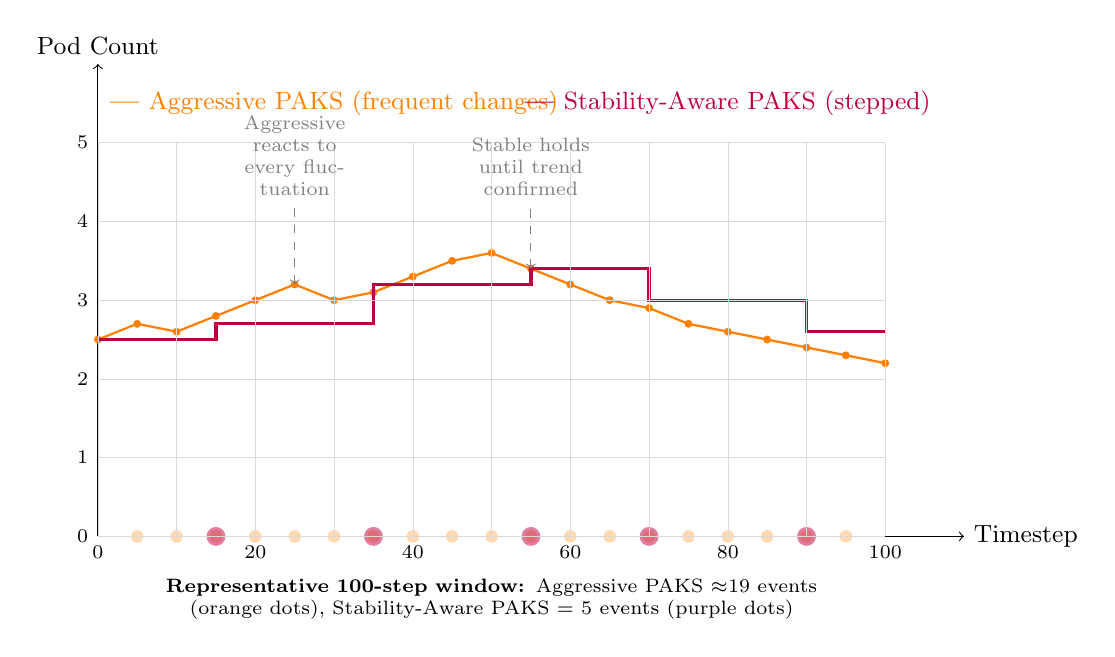
\begin{tikzpicture}[scale=1.0]

% Axes
\draw[->] (0,0) -- (11,0) node[right, font=\small] {Timestep};
\draw[->] (0,0) -- (0,6) node[above, font=\small] {Pod Count};

% Y-axis labels
\foreach \y in {0,1,2,3,4,5} {
  \node[left, font=\scriptsize] at (0, \y) {\y};
}

% X-axis labels (every 20 steps)
\foreach \x in {0,2,4,6,8,10} {
  \node[below, font=\scriptsize] at (\x, 0) {\pgfmathparse{int(\x*10)}\pgfmathresult};
}

% Aggressive PAKS - highly volatile
\draw[thick, orange, mark=*, mark size=1pt] plot coordinates {
  (0,2.5) (0.5,2.7) (1,2.6) (1.5,2.8) (2,3.0) (2.5,3.2) (3,3.0) (3.5,3.1) 
  (4,3.3) (4.5,3.5) (5,3.6) (5.5,3.4) (6,3.2) (6.5,3.0) (7,2.9) (7.5,2.7)
  (8,2.6) (8.5,2.5) (9,2.4) (9.5,2.3) (10,2.2)
};

% Stability-Aware PAKS - stepped with long plateaus
\draw[thick, purple, line width=1.2pt] plot coordinates {
  (0,2.5) (1.5,2.5) (1.5,2.7) (3.5,2.7) (3.5,3.2) (5.5,3.2) (5.5,3.4) 
  (7,3.4) (7,3.0) (9,3.0) (9,2.6) (10,2.6)
};

% Scaling event markers
% Aggressive: many small changes
\foreach \x in {0.5,1,1.5,2,2.5,3,3.5,4,4.5,5,5.5,6,6.5,7,7.5,8,8.5,9,9.5} {
  \fill[orange, opacity=0.3] (\x, 0) circle (0.08);
}

% Stability-Aware: few deliberate steps
\foreach \x in {1.5,3.5,5.5,7,9} {
  \fill[purple, opacity=0.5] (\x, 0) circle (0.12);
}

% Grid for readability
\draw[gray!30, very thin] (0,0) grid[step=1] (10,5);

% Legend
\node[orange, font=\small] at (3, 5.5) {\textbf{---} Aggressive PAKS (frequent changes)};
\node[purple, font=\small] at (8, 5.5) {\textbf{---} Stability-Aware PAKS (stepped)};

% Annotations
\draw[<-, gray, dashed] (2.5, 3.2) -- (2.5, 4.2) node[above, font=\scriptsize, text width=2cm, align=center] {Aggressive\\reacts to\\every fluctuation};

\draw[<-, gray, dashed] (5.5, 3.4) -- (5.5, 4.2) node[above, font=\scriptsize, text width=2cm, align=center] {Stable holds\\until trend\\confirmed};

% Event count annotation
\node[font=\scriptsize, text width=9cm, align=center] at (5, -0.8) {
  \textbf{Representative 100-step window:} Aggressive PAKS $\approx$19 events (orange dots), Stability-Aware PAKS = 5 events (purple dots)
};

\end{tikzpicture}
\caption{Time series of pod count over a representative 100-timestep window. Aggressive PAKS (orange) scales almost continuously in response to prediction fluctuations, exhibiting high volatility. Stability-Aware PAKS (purple) maintains stable plateaus and scales only when sustained demand shifts are detected, resulting in far fewer scaling events (marked as dots on the x-axis).}
\label{fig:scaling_events_timeseries}
\end{figure}
